% ------------------------------------------------------------------------------
% TYPO3 CMS 8.1 - What's New - Chapter "Introduction" (English Version)
%
% @author	Michael Schams <schams.net>
% @license	Creative Commons BY-NC-SA 3.0
% @link		http://typo3.org/download/release-notes/whats-new/
% @language	English
% ------------------------------------------------------------------------------
% LTXE-CHAPTER-UID:		67d83fb2-68e46798-3e745e9b-074bce01
% LTXE-CHAPTER-NAME:	Introduction
% ------------------------------------------------------------------------------

\section{Inleiding}
\begin{frame}[fragile]
	\frametitle{Inleiding}

	\begin{center}\huge{Inleiding}\end{center}
	\begin{center}\huge{\color{typo3darkgrey}\textbf{De feiten}}\end{center}

\end{frame}

% ------------------------------------------------------------------------------
% LTXE-SLIDE-START
% LTXE-SLIDE-UID:		38d75de1-bfa52b35-1853287c-8d0a5fae
% LTXE-SLIDE-ORIGIN:	de1d09f3-1b80b171-45e65f78-cbf750bc English
% LTXE-SLIDE-TITLE:		TYPO3 CMS 8.1 - The Facts
% ------------------------------------------------------------------------------
\begin{frame}[fragile]
	\frametitle{Inleiding}
	\framesubtitle{TYPO3 CMS 8.1 - De feiten}

	\begin{itemize}
		\item Publicatiedatum: 3 mei 2016
		\item Publicatietype: Sprint Release
		\item Slogan: De schroeven aanhalen
	\end{itemize}

	\begin{figure}
		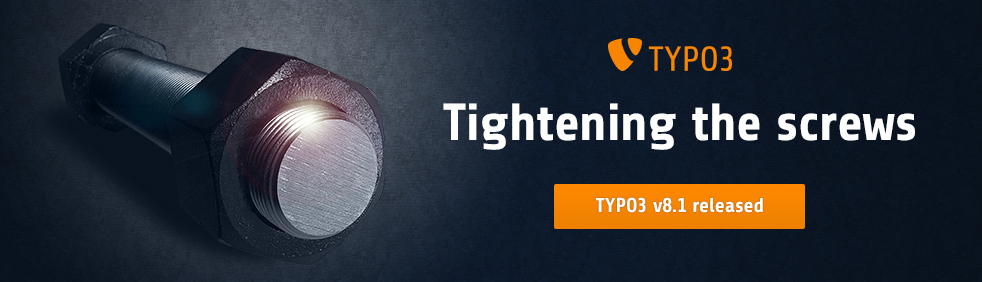
\includegraphics[width=0.95\linewidth]{Introduction/typo3cms81-banner.png}
	\end{figure}

\end{frame}

% ------------------------------------------------------------------------------
% LTXE-SLIDE-START
% LTXE-SLIDE-UID:		86a6e9c1-c158bc50-3331b159-9f85f714
% LTXE-SLIDE-ORIGIN:	29730fa0-cfb7b672-9541b86e-5d979dcc English
% LTXE-SLIDE-TITLE:		System Requirements
% ------------------------------------------------------------------------------
\begin{frame}[fragile]
	\frametitle{Inleiding}
	\framesubtitle{Systeemeisen}

	\begin{itemize}
		\item PHP:\tabto{2.2cm}versie 7
		\item MySQL:\tabto{2.2cm}versie 5.5 to 5.7
		\item Schijfruimte:\tabto{2.2cm}min 200 MB
		\item PHP-instellingen:

			\begin{itemize}
				\item \texttt{memory\_limit} >= 128M
				\item \texttt{max\_execution\_time} >= 240s
				\item \texttt{max\_input\_vars} >= 1500
				\item compilation option \texttt{-}\texttt{-disable-ipv6} mag \underline{niet} gebruikt worden
			\end{itemize}

		\item De backend vereist Microsoft Internet Explorer 11 of nieuwer,
			Microsoft Edge, Google Chrome, Firefox, Safari of een andere moderne
			compatibele browser

	\end{itemize}

\end{frame}

% ------------------------------------------------------------------------------
% LTXE-SLIDE-START
% LTXE-SLIDE-UID:		8c2de61b-e088d5dd-2c18a959-b92c0ddf
% LTXE-SLIDE-ORIGIN:	c5361815-a40c49e2-c6fe93fe-0e0b9466 English
% LTXE-SLIDE-TITLE:		Development And Release Timeline
% ------------------------------------------------------------------------------
\begin{frame}[fragile]
	\frametitle{Inleiding}
	\framesubtitle{Planning voor ontwikkeling en publicatie}

	\begin{figure}
		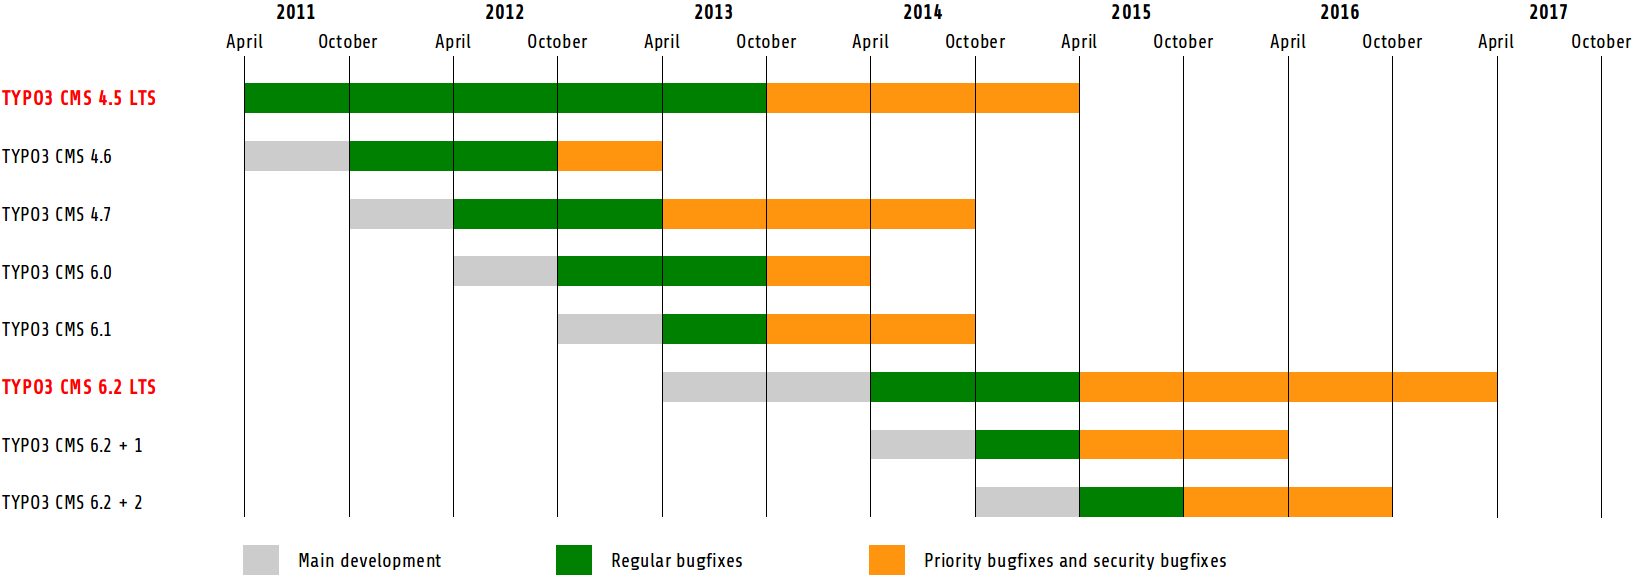
\includegraphics[width=1\linewidth]{Introduction/ReleaseAgenda.png}
	\end{figure}

\end{frame}

% ------------------------------------------------------------------------------
% LTXE-SLIDE-START
% LTXE-SLIDE-UID:		01bf9f7d-2a1c5281-99fb433c-2b36e0a1
% LTXE-SLIDE-ORIGIN:	99e5aeb9-52a34013-e7784c4c-9ff8f701 English
% LTXE-SLIDE-TITLE:		TYPO3 CMS Roadmap
% ------------------------------------------------------------------------------
\begin{frame}[fragile]
	\frametitle{Inleiding}
	\framesubtitle{TYPO3 CMS Roadmap}

	Publicatiedatums en primaire focus:

	\begin{itemize}

		\item v8.0 \tabto{1.1cm}22 mrt 2016\tabto{3.4cm}Last minute toevoegingen
		\item
			\begingroup
				\color{typo3orange}
					v8.1 \tabto{1.1cm}03 mei 2016\tabto{3.4cm}Cloud-itegratie
			\endgroup
		\item v8.2 \tabto{1.1cm}05 jul 2016\tabto{3.4cm}Rich Text Editor
		\item v8.3 \tabto{1.1cm}30 aug 2016\tabto{3.4cm}Bewerken in Frontend powereditie
		\item v8.4 \tabto{1.1cm}18 okt 2016\tabto{3.4cm}\textit{onbekend}
		\item v8.5 \tabto{1.1cm}20 dec 2016\tabto{3.4cm}Integrator-ondersteuning
		\item v8.6 \tabto{1.1cm}14 feb 2017\tabto{3.4cm}\textit{onbekend}
		\item v8.7 \tabto{1.1cm}04 apr 2017\tabto{3.4cm}LTS Voorbereiding

	\end{itemize}

	\smaller
		\url{https://typo3.org/typo3-cms/roadmap/}\newline
		\url{https://typo3.org/news/article/kicking-off-typo3-v8-development/}
	\normalsize

\end{frame}

% ------------------------------------------------------------------------------
% LTXE-SLIDE-START
% LTXE-SLIDE-UID:		9cc25fa2-75412937-7736a93f-13d559b2
% LTXE-SLIDE-ORIGIN:	3159ba35-9542333b-a0495cfc-af0010a5 English
% LTXE-SLIDE-TITLE:		Installation
% ------------------------------------------------------------------------------
\begin{frame}[fragile]
	\frametitle{Inleiding}
	\framesubtitle{Installatie}

	\begin{itemize}
		\item Officiële installatieprocedure op Linux/Mac OS X\newline
			(DocumentRoot bijvoorbeeld \texttt{/var/www/site/htdocs}):
		\begin{lstlisting}
			$ cd /var/www/site
			$ wget --content-disposition get.typo3.org/8.1
			$ tar xzf typo3_src-8.1.0.tar.gz
			$ cd htdocs
			$ ln -s ../typo3_src-8.1.0 typo3_src
			$ ln -s typo3_src/index.php
			$ ln -s typo3_src/typo3
			$ touch FIRST_INSTALL
		\end{lstlisting}

		\item Symbolische links op Microsoft Windows:

			\begin{itemize}
				\item Gebruik \texttt{junction} op Windows XP/2000
				\item Gebruik \texttt{mklink} op Windows Vista en Windows 7
			\end{itemize}

	\end{itemize}
\end{frame}

% ------------------------------------------------------------------------------
% LTXE-SLIDE-START
% LTXE-SLIDE-UID:		45e2bad0-1dafa193-a9f5ec5a-8122d874
% LTXE-SLIDE-ORIGIN:	d3497bd8-61e5242f-0009b322-3a285ed7 English
% LTXE-SLIDE-TITLE:		Upgrade to TYPO3 CMS 7
% ------------------------------------------------------------------------------
\begin{frame}[fragile]
	\frametitle{Inleiding}
	\framesubtitle{Upgrade naar TYPO3 CMS 8.x}

	\begin{itemize}
		\item Upgrades alleen mogelijk vanaf TYPO3 CMS 7.6 LTS
		\item TYPO3 CMS < 7.6 LTS moet eerst naar TYPO3 CMS 7.6 LTS bijgewerkt worden
	\end{itemize}

	\begin{itemize}

		\item Upgrade-instructies:\newline
			\smaller\url{http://wiki.typo3.org/Upgrade#Upgrading_to_8.1}\normalsize
		\item Officiële TYPO3-handleiding "TYPO3 Installation and Upgrading":
			\smaller\url{http://docs.typo3.org/typo3cms/InstallationGuide}\normalsize
		\item Algemene aanpak:
			\begin{itemize}
				\item Controleer minimale systeemeisen \small(PHP, MySQL, etc.)
				\item Bekijk \textbf{deprecation\_*.log} in oude TYPO3 installatie
				\item Update alle extensies naar laatste versie
				\item Zet nieuwe broncode neer en start Install Tool -> Upgrade Wizard
				\item Bekijk startmodule voor backend gebruikers (optioneel)
			\end{itemize}
	\end{itemize}

\end{frame}

% ------------------------------------------------------------------------------

% ------------------------------------------------------------------------------
% LTXE-SLIDE-START
% LTXE-SLIDE-UID:		95eaea01-ba5b5013-cc3879c9-727bb2b1
% LTXE-SLIDE-ORIGIN:	31bb3281-23ea7e95-5ed92903-61de52e7 English
% LTXE-SLIDE-TITLE:		PHP Version 7
% ------------------------------------------------------------------------------
\begin{frame}[fragile]
	\frametitle{Inleiding}
	\framesubtitle{PHP Versie 7}

	\begin{itemize}

		\item PHP 7.0 is de minimale eis voor TYPO3 CMS 8.x
		\item TYPO3 zal volgende PHP 7 versies ondersteunen wanneer deze uitkomen
		\item Deze versie geeft significant meer prestaties op het hele systeem

		\item Niet alleen backendgebruikers merken een soepelere interface, maar ook het
			nieuwe record voor een volledig gecachete pagina in de frontend is nu minder
			dan 7 milliseconden, wat ongeveer 40\% sneller is in vergelijking met dezelfde
			website met PHP versie 5.5

		\item We zijn ook begonnen nieuwe features van deze PHP-versie te gebruiken, bijvoorbeeld
			de cryptografisch veilige pseudo-random generatoren worden al ingezet

	\end{itemize}

\end{frame}

% ------------------------------------------------------------------------------
